\chapter{Results and discussion}
\label{chap:results}
In this chapter, we present the results of our experiments.
When comparing tasks performance, we implicitly use F1 Macro, as
all tasks but Day Of Week are imbalanced. We start with an overall
comparison of the models. We then perform a closer analysis of the
individual tasks and put them into the context of the related research.

\section{Results}
\subsection{Human Agreement and Performance}
\label{sec:results}
\begin{table}[h]
    \resizebox{\linewidth}{!}{%
        \centering\footnotesize\sf
        \begin{tabular}{lrrrrrrrr}
            \toprule
            {}    & \multicolumn{2}{l}{Server} & \multicolumn{2}{l}{Category} & \multicolumn{2}{l}{Gender} & \multicolumn{2}{l}{Day of week}                                                                     \\
            {}    & F1-macro                   & F1-micro                     & F1-macro                   & F1-micro                        & F1-macro       & F1-micro       & F1-macro       & F1-micro       \\
            \midrule
            Human & 27.03                      & 30.25                        & 40.26                      & 60.76                           & 50.09          & 61.75          & 13.53          & 13.75          \\
            Final & \textbf{71.22}             & \textbf{80.00}               & \textbf{52.04}             & \textbf{79.59}                  & \textbf{52.79} & \textbf{79.00} & \textbf{28.37} & \textbf{29.00} \\
            \bottomrule
        \end{tabular}
        \caption{Results on the Human Test set. We use bold to denote the best result for each task.}
        \label{tab:results-human}
    }
\end{table}
\label{sec:human-baseline}
We found the average Cohen's kappa to be: 0.08 for Server, 0.65 for Category,
0.20 for Gender and 0.01 for Day Of Week. Based on the classification from \autoref{sec:interannotator},
only the category task showed at least substantial agreement.

The performance results presented in \autoref{tab:results-human}
shows that the final models significantly outperform the human baseline.
The largest difference, a 44 percent improvement, was observed
on the Server task.

Overall, low agreement and performance suggest the high difficulty of the tasks.


\begin{table}[h]
    \resizebox{\linewidth}{!}{%
        \centering\footnotesize\sf
        \begin{tabular}{lrrrrrrrr}
            \toprule
            {}       & \multicolumn{2}{l}{Server} & \multicolumn{2}{l}{Category} & \multicolumn{2}{l}{Gender} & \multicolumn{2}{l}{Day of week}                                                                     \\
            {}       & F1-macro                   & F1-micro                     & F1-macro                   & F1-micro                        & F1-macro       & F1-micro       & F1-macro       & F1-micro       \\
            \midrule
            LR-50    & 36.92                      & 52.78                        & 33.30                      & 72.32                           & 43.62          & 69.15          & 18.13          & 19.62          \\
            LR-200   & 37.27                      & 53.38                        & 32.77                      & 72.69                           & 44.06          & 69.83          & 18.34          & 19.97          \\
            \addlinespace
            R-Base   & 69.74                      & 78.19                        & 54.35                      & 79.67                           & 51.18          & 74.67          & 29.43          & 29.49          \\
            F-Base   & 69.39                      & 77.68                        & 53.97                      & 79.55                           & -              & -              & 29.24          & 29.34          \\
            \addlinespace
            R-Small  & 59.48                      & 67.85                        & 36.55                      & 77.46                           & 44.97          & 69.95          & 17.42          & 19.61          \\
            F-Small  & -                          & -                            & 37.84                      & 77.72                           & -              & -              & 16.08          & 17.99          \\
            \addlinespace
            Truncate & 68.71                      & 77.31                        & 53.90                      & 79.37                           & 50.36          & 74.21          & 29.52          & 29.57          \\
            LM-tune  & 70.06                      & 78.40                        & 55.18                      & 80.14                           & 51.13          & \textbf{75.09} & \textbf{29.98} & \textbf{30.00} \\
            Grad-12  & 67.81                      & 76.36                        & 51.93                      & 78.69                           & 49.98          & 73.82          & 29.11          & 29.21          \\
            Grad-24  & 69.07                      & 77.69                        & 53.22                      & 78.97                           & 49.75          & 74.06          & 29.36          & 29.47          \\
            \midrule
            Final    & \textbf{71.04}             & \textbf{79.25}               & \textbf{56.06}             & \textbf{80.47}                  & \textbf{51.94} & 75.04          & 29.68          & 29.69          \\
            \bottomrule
        \end{tabular}
        \caption{Results on the Test set. We use - to denote a failure of a model to converge for all tested learning rates.}
        \label{tab:results-test}
    }
\end{table}

\subsection{Baseline Model}
\label{sec:baseline}
The baseline model results are shown in \autoref{tab:results-test}.
A tiny improvement was gained by adding the additional 150k features.
\autoref{ch:baseline_features} shows the features with the highest weights for each task and class,
adding insight into the model's reasoning process.


\subsection{Pre-trained Transformers}
\autoref{tab:results-test} shows a significant improvement in Pre-trained transformer models over
Logistic Regression across the tasks. This demonstrates the importance of capturing textual dependencies for better performance.
Contrary to the initial expectation that Fernet-News would achieve higher
scores due to its same-domain training data, RobeCzech outperformed Fernet-News across the tasks.
One possible explanation could be RobeCzech's slightly
higher capacity, which may be more important for long training.
\begin{table}[h]
    \resizebox{\linewidth}{!}{%
        \centering\footnotesize\sf
        \begin{tabular}{lrrrrrrrr}
            \toprule
            {}      & \multicolumn{2}{l}{Server} & \multicolumn{2}{l}{Category} & \multicolumn{2}{l}{Gender} & \multicolumn{2}{l}{Day of week}                                                                     \\
            {}      & F1-macro                   & F1-micro                     & F1-macro                   & F1-micro                        & F1-macro       & F1-micro       & F1-macro       & F1-micro       \\
            \midrule
            R-Base  & \textbf{78.43}             & \textbf{82.88}               & \textbf{56.17}             & \textbf{80.65}                  & \textbf{52.38} & \textbf{75.61} & \textbf{27.96} & \textbf{28.33} \\
            F-Base  & 78.04                      & 82.26                        & 55.51                      & 80.51                           & -              & -              & 27.25          & 27.78          \\
            \addlinespace
            R-Small & 75.12                      & 80.37                        & 37.88                      & 77.69                           & 47.45          & 74.30          & 17.41          & 19.82          \\
            F-Small & -                          & -                            & 39.31                      & 77.88                           & -              & -              & 17.68          & 19.20          \\
            GPT-3   & 67.30                      & 73.12                        & 44.76                      & 75.21                           & 42.92          & 70.28          & 19.49          & 20.83          \\
            \bottomrule
        \end{tabular}
        \caption{Results on the Test Small. We use - to denote
            a failure of a model to converge for all tested learning rates.}
        \label{tab:results-small}
    }
\end{table}

The Small train setting yielded opposite results as seen in \autoref{tab:results-small}.
For every task where F-Small didn't diverge, it outperformed R-Small.
The dominance of Fernet-News in the Small setting could be explained by
better weights initialization, as the domain of the data is the same
in the case of Fernet-News unlike in RobeCzech. Compared to the fully
trained models, small models showed great results considering that they were trained on less than 6\% of the data.
However, it is apparent that further training is beneficial~(\autoref{tab:results-test}).

Regarding GPT-3, it outperformed both Small models on Category and Day of Week, showing its multi-lingual capabilities.
The model exhibited the tokenization issues of multilingual models~(\autoref{sec:multilinguality}).
It tokenized just 1.77 characters per token compared to
4.68 and 4.46 in the case of RobeCzech and Fernet-News, making the training more expensive than expected.
Overall we spent around 40\$ for both training and inference.

Surprisingly, we observed better Server task results of the models on the Test Small.
The underlying reason for this observation remains unclear, especially considering
that the distributions are relatively similar across the test sets. The only
noticeable change is iDnes.cz having slightly higher representation at the expense
of Deník.cz.


\subsection{Fine-tuning Enhancements}
\begin{figure}[ht]
    \centering
    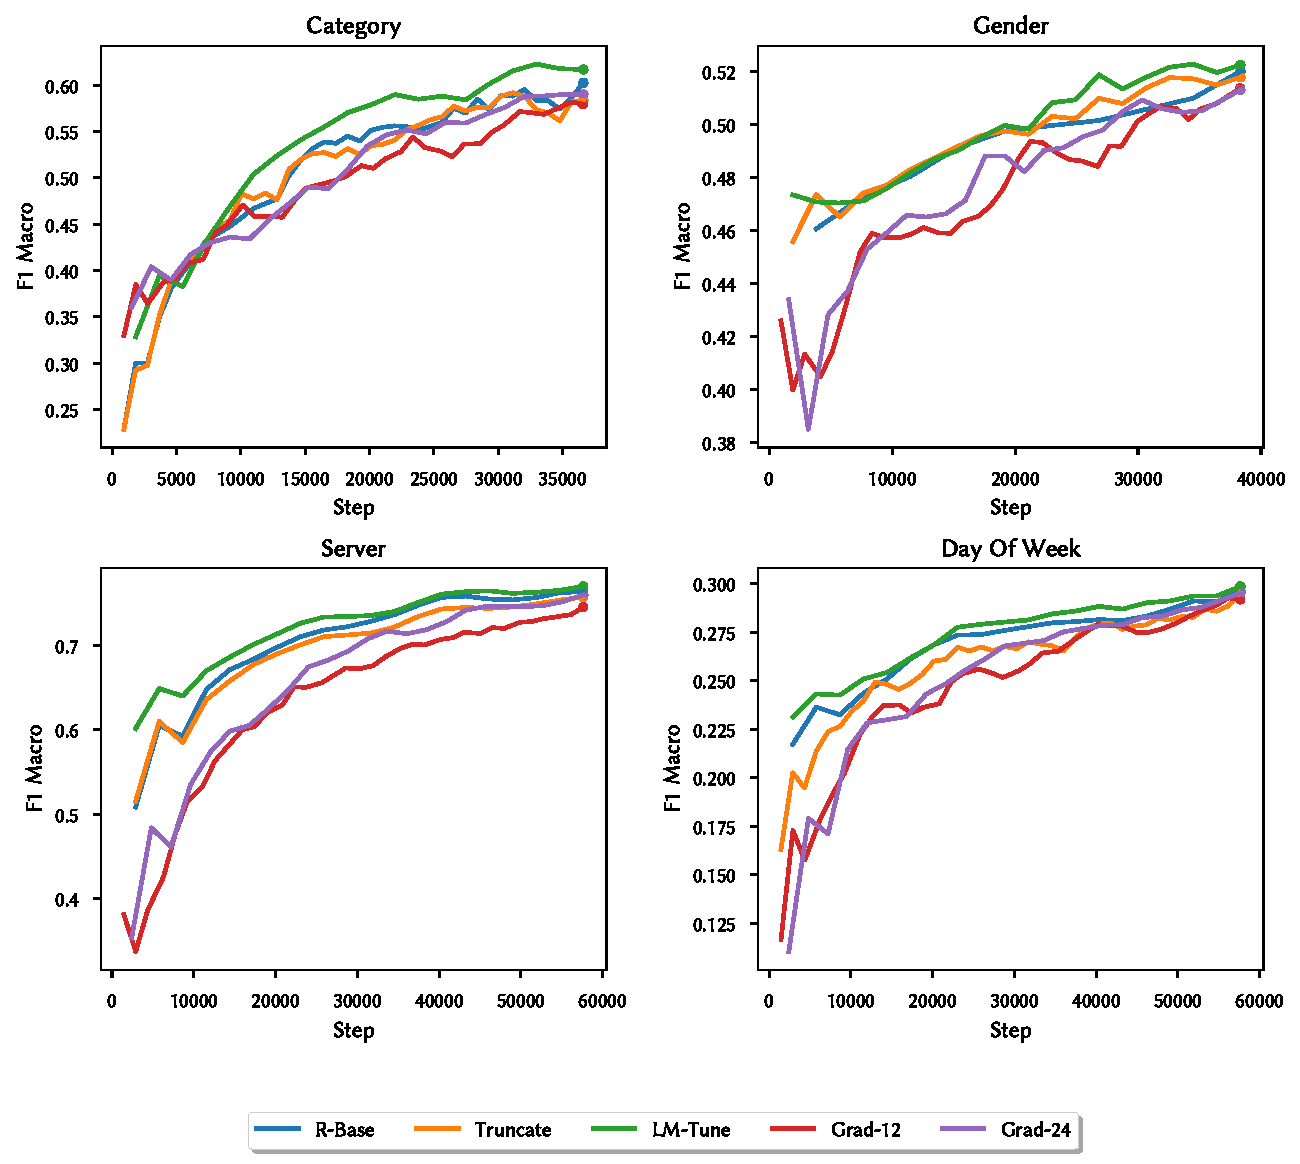
\includegraphics[width=1.0\textwidth]{graph_create/outputs/tune.pdf}
    \caption{Validation curves for all tasks and fine-tuning approaches. The curves are displayed
        with linear smoothing. Each Validation was run on 10\% of the Validation set. The last validation
        was run on the whole Validation set.}
    \label{fig:vallidation-curves-tune}
\end{figure}
Article beginning truncation didn't help the performance, as seen in~\autoref{fig:vallidation-curves-tune}.
The same was observed with \ac{gu}, which even significantly worsened the performance
in some cases. From validation curves, we can observe that in all tasks but Category,
\ac{gu} performance falls behind considerably at the beginning of the training and
catches up only at the end.
That is caused by the different alignment of the tasks with the Language Modelling objective.
Since the weights of lower layers are frozen at the start,
good initialization is needed to keep up with the fully-unfrozen model.
The only positive aspect of \ac{gu} was smaller memory consumption at early training stages,
allowing for larger batch sizes.

Out of all fine-tuning approaches, only \ac{flm} increased the performance.

\subsection{Final Model}
\label{sec:final-model-performance-on-tasks}
The performance of the Final model can be seen in~\autoref{tab:results-test}.
It shows the importance of further pretraining and recency sampling.

\section{Tasks Evaluation}
We selected the Final model for in-depth evaluation of all tasks, even
though it wasn't the best-performing model for Day Of Week.


\subsection{Server}
\label{sec:final-model-performance-on-server}
\begin{table}[h]
    \centering\footnotesize\sf
    \begin{tabular}{lrrr}
        \toprule
        {}              & Precision & Recall & F1    \\
        \midrule
        SeznamZprávy.cz & 82.44     & 65.06  & 72.72 \\
        iDnes.cz        & 68.56     & 75.60  & 71.91 \\
        Aktuálně.cz     & 83.08     & 81.30  & 82.18 \\
        Novinky.cz      & 29.64     & 67.75  & 41.23 \\
        Deník.cz        & 91.75     & 86.39  & 88.99 \\
        iRozhlas.cz     & 60.43     & 80.95  & 69.20 \\
        Macro Avg       & 69.32     & 76.17  & 71.04 \\
        \bottomrule
    \end{tabular}
    \caption{Classification report of Server on Test set.}
    \label{tab:classification-report-server}
\end{table}
To our knowledge, there is no previous work on the Server task. Therefore our only comparison
is to human performance, which was outperformed by the model significantly.

We observed the most problematic origin to be Novinky.cz. The model
incurs a significant precision drop on this origin as seen in \autoref{tab:classification-report-server}.
This could be explained by the distribution change in a train and test set.
Compared to the training set, the test set contains a smaller number of samples from Novinky.cz.
Overpredicting Novinky.cz is then natural behavior. The opposite was observed with SeznamZprávy.cz.
The model misclassifies underrepresented SeznamZprávy.cz mainly as iDnes.cz~(\autoref{fig:server-conf}), which results in
a low recall.

\subsection{Category}
\label{sec:final-model-performance-on-category}
\begin{table}[h]
    \centering\footnotesize\sf
    \begin{tabular}{lrrr}
        \toprule
        {}                     & Precision & Recall & F1    \\
        \midrule
        World                  & 82.62     & 86.77  & 84.65 \\
        Home                   & 86.89     & 82.91  & 84.86 \\
        Sport                  & 97.78     & 97.97  & 97.87 \\
        Culture                & 58.07     & 87.26  & 69.73 \\
        Celebrity              & 81.91     & 67.78  & 74.18 \\
        Gossip and Curiosities & 28.08     & 45.34  & 34.68 \\
        Economics              & 51.35     & 65.99  & 57.76 \\
        Crime                  & 60.58     & 62.30  & 61.43 \\
        Entrepreneurship       & 28.68     & 51.80  & 36.92 \\
        Car                    & 85.45     & 86.31  & 85.88 \\
        Science                & 54.35     & 51.48  & 52.87 \\
        Comments               & 68.88     & 85.70  & 76.38 \\
        Travel                 & 36.83     & 39.55  & 38.14 \\
        Finance                & 60.21     & 59.44  & 59.82 \\
        Technology             & 79.76     & 82.70  & 81.20 \\
        Housing                & 67.56     & 75.69  & 71.39 \\
        Coronavirus            & 42.72     & 33.24  & 37.39 \\
        Business               & 62.78     & 51.72  & 56.71 \\
        Interviews             & 7.95      & 8.64   & 8.28  \\
        Podcasts               & 0.00      & 0.00   & 0.00  \\
        Lifestyle              & 53.12     & 46.00  & 49.30 \\
        Literature             & 90.24     & 82.68  & 86.30 \\
        Christmas              & 11.11     & 25.00  & 15.38 \\
        Fine Arts              & 92.19     & 71.08  & 80.27 \\
        Bicycle                & 0.00      & 0.00   & 0.00  \\
        Macro Avg              & 55.57     & 57.89  & 56.06 \\
        \bottomrule
    \end{tabular}
    \caption{Classification report of Category on the Test set.}
    \label{tab:classification-report-category}
\end{table}
The Category was researched in the works of \cite{sunagar2021news} and \cite{fuksClassificationNewsDataset2018}.
In the first work, the authors report 90.85\% F1 Micro; however, the authors only used four categories from a single source.
The second work is more comparable as the authors used the same number of categories (25) but from a single source.
The authors report 68.38\% F1 Micro. We thus find our results reasonably good.

When observing the results(~\autoref{tab:classification-report-category}, \autoref{fig:category-conf})
we noticed our preprocessing likely made the task harder. For example,
the model often misclassified Fine Arts and Literature as Culture, due to Culture being a parent category of both.
Similar could be observed with Business, Entrepreneurship and Finance being mistaken for Economy.

Additionally, we found that the model often misclassified Coronavirus as Home.
When looking at the data,
we found that some servers do not have the category Coronavirus and rather classify the article as Home,
since the topic of the article is often also about politics. This yields a question
evaluation in a single-label setting, as often the articles could be classified into multiple categories.

\subsection{Gender}
\begin{table}[h]
    \centering\footnotesize\sf
    \begin{tabular}{lrrr}
        \toprule
        {}        & Precision & Recall & F1    \\
        \midrule
        Man       & 82.70     & 78.73  & 80.67 \\
        Woman     & 63.79     & 72.22  & 67.75 \\
        Mixed     & 23.89     & 4.38   & 7.41  \\
        Macro Avg & 56.79     & 51.78  & 51.94 \\
        \bottomrule
    \end{tabular}
    \caption{Classification report of Gender on Test set.}
    \label{tab:classification-report-gender}
\end{table}
Gender task has also been studied in a few works such as by \cite{haagsma2019overview}
. The paper is a results overview of the shared gender classification task in Dutch.
The data are gathered from multiple Dutch news sources but
don't consider multi-author articles. Authors report 68.9\% F1 Micro for the best model.
This makes our results look great. Note, however, that the language difference could play
a huge role.

Confusion matrix~(\autoref{fig:gender-conf}) and classification report~(\autoref{tab:classification-report-gender})
show that the Mixed class is highly problematic for the model, which likely stems from low data representation.
When it comes to Man and Woman comparison, we observed Woman to have both precision and recall smaller. While we expected
the recall to be smaller, due to imbalance, we didn't expect the precision to be lower as well.
\subsection{Day of week}
\begin{table}[h]
    \centering\footnotesize\sf
    \begin{tabular}{lrrr}
        \toprule
        {}        & Precision & Recall & F1    \\
        \midrule
        Monday    & 30.08     & 34.02  & 31.93 \\
        Tuesday   & 27.69     & 28.23  & 27.95 \\
        Wednesday & 30.28     & 27.57  & 28.86 \\
        Thursday  & 25.45     & 34.57  & 29.32 \\
        Friday    & 33.22     & 28.60  & 30.73 \\
        Saturday  & 34.86     & 22.63  & 27.44 \\
        Sunday    & 33.95     & 29.37  & 31.49 \\
        Macro Avg & 30.79     & 29.28  & 29.68 \\
        \bottomrule
    \end{tabular}
    \caption{Classification report of Day Of Week on Test set.}
    \label{tab:classification-report-day}
\end{table}
No such study of the task is known to us. We anticipated the task to be the most challenging one,
which was shown to be true by the lowest agreement and performance by humans among the tasks. Considering
the human results, we find our results excellent.

From the confusion matrix~(\autoref{fig:day-conf}), we can see the model misclassifying the days
as surroundings of the target day. The only exception to this rule
is weekend days. This can be observed with both Monday and Friday, as they are
rather misclassified as random weekdays rather than surrounding Sunday, respectively
Saturday.